\chapter{Технологический раздел}
\label{ch:tech}
В данном разделе описываются использованные технологии разработки, сборки и публикации, отладки и тестирования Android-приложений.

\section{Разработка под Android}
\label{sec:dev}

\subsection{Архитектура приложения}
\label{subsec:arch}

Чаще всего Android-разработчиками используется подход под названием ``Clean Architecture'' или ``чистая архитектура''.
Изначально подход был сформулирован Бобом Мартином еще в 2012 году\cite{martin:clean} и использовался не только в Android-разработке.
Основная идея подхода состоит в том, чтобы написать приложение, которое:
\begin{itemize}
  \item не зависит от пользовательского интерфейса;
  \item не зависит от внешних ферймворков, хранилища информации и библиотек;
  \item легко тестируется.
\end{itemize}

Таким образом, в хорошо спроектированном приложении можно ``откладывать'' решения до того момента, когда их действительно необходимо принять.
Если вместо одной технологии хранения появится другая более привлекательная, или если используемая технология перестанет справляться с нагрузкой "--- возможность лёгкой смены решения сыграет на руку.
В итоге получается слоистая и гибкая архитектура, единый подход в осмыслении всего приложения~\cite{gihub:androidArch}.

\begin{figure}[ht]
  \centering
  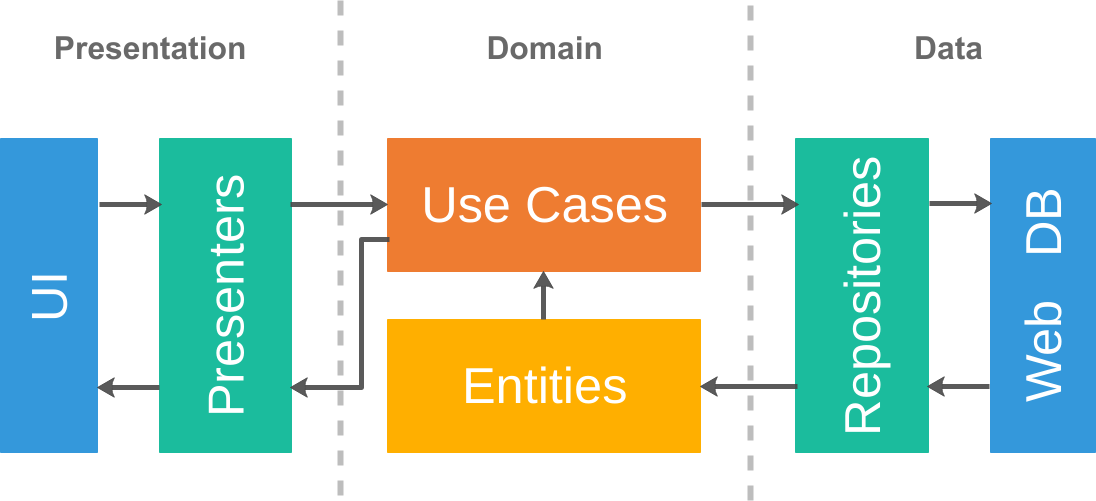
\includegraphics[width=\textwidth]{inc/img/clean_arch.png}
  \caption{Линейная диаграмма, изображающая слои чистой архитектуры}
  \label{fig:cleanArch}
\end{figure}

Изначально Роберт Мартин изобразил архитектуру как четырёхслойную ``луковицу'', у которой в центре находится слой Entity, а снаружи UI, Web, DB, но удобнее представлять чистую архитектуру в виде линейной диаграммы, изобрженной на рисунке~\ref{fig:cleanArch}.

Стрелки показывают потоки данных между слоями.
Например, событие, инициированное пользователем, идет в Presenter, тот образается к Use Case.
Use Case делает запрос в Repository, который получает данные, создает Entity и передает его в UseCase.
Так Use Case получает все нужные ему Entity.
Затем, применив их и свою логику, получает результат, который передает обратно в Presenter.
А тот, в свою очередь, отображает результат в UI~\cite{habr:clean}.

Разработку приложения удобнее вести сверху вниз, то есть сначала реализовывать внешние слои и постепенно углубляться в внутренним.
Это позволяет максимально быстро увидеть результат, кроме того, всегда удобно отталкиваться от того, что должен видеть пользователь.

Как видно из рисунка~\ref{fig:cleanArch}, проект удобно делить на три части: presentation, domain и data.
Модуль presentation зависит от Android API, так как взаимодействует с графическим интерфейсом и прочими функциями системы.
Слой data, так же, частично зависит от Android API т.к. в нём происходит взаимодействие с сетью, файлами и базами данных.
Слой domain напротив полностью независим от Android и в нём содержится вся бизнес-логика приложения.

\subsection{Структура проекта}
\label{subsec:struct}

Есть два типа разбиения структуры проекта: по слоям и по возможностям (или функциям).
При разбиении проекта по слоям возникает риск захламлённости пакетов, т.к. при использовании чистой архитектуры количество классов увеличивается довольно быстро.
Разбиение по возможностям, мало того, что лишено этого недостатка, но еще и обладает дополнительными преимуществами:
\begin{enumerate}
  \item Можно узнать о возможностях приложения только посмотрев на структуру папок;
  \item Легко добавлять новые возможности в приложение;
  \item Легко удалять возможности, для этого достаточно лишь удалить директорию;
  \item Легко ориентироваться в коде, когда он организован таким образом;
  \item Позволяет переиспользовать код в других проектах;
  \item Разработчики могут работать независимо друг от друга в разных пакетах~\cite{medium:pbf}.
\end{enumerate}

\begin{figure}[!ht]
  \minipage[b]{0.32\textwidth}
    \begin{forest}
      [\textbf{Presentation}
        [internal
          [di]
        ]
        [presentation
          [feature
            [activity]
            [fragment]
            [presenter]
            [\textit{view}]
          ]
        ]
        [utils]
      ]
    \end{forest}
    \caption{Структура модуля Presentation}\label{fig:presentationStruct}
  \endminipage\hfill
  \minipage[b]{0.32\textwidth}
    \begin{forest}
      [\textbf{Domain}
        [model]
        [\textit{repository}]
        [usecase]
        [utils]
      ]
    \end{forest}
    \caption{Структура модуля Domain}\label{fig:domainStruct}
  \endminipage\hfill
  \minipage[b]{0.32\textwidth}%
    \begin{forest}
      [\textbf{Data}
        [converter]
        [entity]
        [network]
        [repository]
        [storage]
        [utils]
      ]
    \end{forest}
    \caption{Структура модуля Data}\label{fig:dataStruct}
  \endminipage
\end{figure}

При разбивке проекта по возможностям, структура проекта имеет вид как на рисунках~\ref{fig:presentationStruct}--\ref{fig:dataStruct}, где жирным шрифтом выделены названия модулей, а курсивом директории, которые содержат абстрактные сущности.

\section{Сборка и публикация приложения}
\label{sec:build}

\subsection{Система автоматической сборки Gradle}
\label{subsec:gradle}

\Abbrev{APK}{Android package kit}
\Abbrev{DSL}{domain-specific language "--- язык, специфический для предметной области}
\Abbrev{XML}{extensible markup language "--- расширяемый язык разметки}
Для сборки приложения в APK файл при Android-разработке обычно используется Gradle.
Это система автоматизации сборки с открытым исходным кодом, ориентированная на гибкость и производительность.
В отличие от аналогов (Maven и Ant), сценарии сборки пишутся на Groovy или Kotlin DSL, а не на XML\@.
Это позволяет максимально снизить порог вхождения для программиста~\cite{gradle:docs}.

Gradle является официальным инструментом сборки для Android и поддерживает многие популярные языки и технологии.
Время сборки сильно уменьшается за счёт того, что при сборке используются результаты прошлых сборок, выполняется сборка только измененных файлов (инкрементальная сборка) и независимые между собой задачи выполняются параллельно.
Gradle поддерживается всеми IDE для Android-разработки, в том числе IntelliJ IDEA\@.

При создании нового проекта в IDEA можно выбрать какой DSL использовать для сценариев сборки.
В процессе разработки МП СУПС используется Kotlin DSL, т.к. язык проекта "--- Kotlin.
После указания основных настроек (название приложения, домен, целевая версия и т.д.) создаются стандартные сценарии сборки для всего проекта и для модуля 'app', в котором содержится код приложения.
Это обусловлено тем, что в проекте может быть несколько модулей, например, модули data, domain и presentation при использовании чистой архитектуры.
Gradle и Kotlin DSL обновляются чаще чем инструменты разработки Android, поэтому созданные по умолчанию сценарии сборки могут не работать в силу того, что Kotlin DSL находится в стадии активной разработки и не гарантирует обратную совместимость, а шаблоны рассчитаны на старые версии.

Помимо сценариев сборки в Gradle есть еще файлы настроек:
\begin{itemize}
  \item \code{gradle.properties} содержит настройки Gradle (здесь, например, можно выставить ограничение потребления памяти);
  \item \code{settings.gradle.kts} содержит список модулей, которые нужно подключить;
  \item \code{gradle-wrapper.properties} (находится по пути \code{gradle/wrapper/}) содержит настройки обёртки Gradle (Gradle wrapper).
\end{itemize}

Gradle позволяет дописывать собственные вспомогательные классы, которые можно будет использовать при написании сценария сборки.
Такие классы помещают в модуль \code{buildSrc}, который подключён по умолчанию и этот собирается перед сборкой остальных модулей.
Еще одна возможность организации структуры сценариев сборки "--- разбивка сценария на несколько файлов, отвечающих за разные аспекты сборки.
Например, выделить отдельный файл, в котором будет собрана вся работа с зависимостями.
В Gradle для подключения внешних файлов сценариев предусмотрена функция:
\codeline{kotlin}{project.apply { from("path/to/script.gradle.kts") }}

Все необходимые задачи, такие как настройка проекта для работы с Android, сборка приложения в APK, подпись его ключом и пр.\ выделены в отдельный плагин "--- Android Gradle Plugin.
Подключение этого плагина осуществляется в сценарии уровня проекта в секции \code{buildscript.dependencies} (листинг~\ref{lst:rootBuildKts}).

\begin{listing}[H]
  \kotlinfile{inc/src/rootBuild.gradle.kts}
  \caption{Подключение Android Gradle Plugin версии 3.0.1}
  \label{lst:rootBuildKts}
\end{listing}

После того, как плагин подключен, в сценарии уровня модуля, нужно указать настройки сборки Android приложения, а именно, целевую версию, минимальную допустимую версию, версию инструментов сборки, ID и версию приложения (листинг~\ref{lst:moduleBuildKts}).

\begin{listing}[H]
  \kotlinfile{inc/src/moduleBuild.gradle.kts}
  \caption{Настройка сборки Android-приложения}
  \label{lst:moduleBuildKts}
\end{listing}

\subsection{Управление зависимостями}
\label{subsec:libs}

Ни одно Android-приложение не обходится без зависимостей.
Проект всегда использует бибилиотеки, а так же может быть разбит на отдельные модули, которые зависят друг от друга.
Управление зависимостями "--- это метод декларирования, разрешения и использования зависимостей, требуемых проектом в автоматическом режиме.

В Gradle есть инструменты для управления зависимостями, которые покрывают все типичные сценарии, встречающиеся в современных проектах по разработке ПО\@.

\todo{Картинка управления зависимостями в Gradle}

Например есть проект, написанный на Java.
В некоторых файлах используются классы из Google Guava (библиотека с открытым исходным кодом, предоставляющая множество полезных функций).
Кроме того, проекту нужен JUnit для компиляции и выполнения тестов.

Guava и JUnit представляют собой зависимости этого проекта.
Программист, при написании сценария сборки, может определять зависимости для разных областей (scopes), например, для компиляции всего кода или для компиляции и выполнения тестов.
В Gradle область действия зависимости называется ``конфигурацией''.

Обычно зависимости подключаются в виде модулей.
Необходимо указать Gradle, где найти эти модули, чтобы их можно было использовать во время сборки.
Место хранения модулей называется репозиторием.
После указания репозиториев для сборки, Gradle будет знать, как находить и получать модули.
Репозитории могут быть разных типов: локальный каталог и удаленный или локальный репозиторий.
Для обеспечения совместимости с популярными хранилищами модулей Gradle может использовать Maven и Ivy репозитории

Gradle определяет требуемые зависимости во время выполнения сценария сборки.
Зависимости могут быть загружены из удаленного репозитория, извлечены из локального каталога или могут потребовать сборки другого проекта при многопроектной конфигурации.
Этот процесс называется разрешением зависимостей.

После разрешения Gradle хранит файлы зависимости в локальном кэше, называемом кэшем зависимостей.
При повторной сборке будут повторно использованы файлы, хранящиеся в кэше, чтобы избежать ненужных сетевых вызовов и ускорить сборку.

Модули могут предоставлять метаданные, то есть данные, которые дополнительно описывают модуль, например, координаты для нахождения его в репозитории, актуальную версия модуля, информацию об авторах и т.д.
В рамках метаданных модуль может объявить, что для его работы необходимы другие модули, а Gradle автоматически разрешает эти дополнительные зависимости, которые называют ``транзитивными зависимостями''.

Проекты с большим количеством зависимостей могут пострадать от антипаттерна, называемого ``ад зависимостей'' (dependency hell).
Для борьбы с этим Gradle предоставляет инструментарий для визуализации и анализа графа зависимостей проекта.

\subsubsection*{Объявление зависимостей}

Типичным примером библиотеки в Java-проекте является JUnit 4 (в Kotlin-проекте эта библиотека может быть заменена модулем \code{kotlin-test-junit}).

\begin{listing}[H]
  \kotlinfile[escapeinside=||]{inc/src/junitDependency.gradle.kts}
  \caption{Подключение JUnit 4 в качестве зависимости}
  \label{lst:junitDependency}
\end{listing}

В листинге~\ref{lst:junitDependency} приведен пример кода, который подключает JUnit в проект как зависимость для сборки и выполнения тестов.
В строке~\ref{line:repo} подключается репозиторий Maven Central, в котором находится модуль JUnit.
В строке~\ref{line:junit} происходит объявление самого JUnit, для этого указываются координаты артефакта в формате \code{<group>:<module>:<version>}.
В начале строки указана область действия зависимости или, в терминологии Gradle, конфигурация "--- \code{testImplementation}.
Существует много различных конфигураций, но самые часто используемые это \code{implementation} и \code{testImplementation}.
В первом случае зависимость используется для компиляции всего проекта, во втором только для компиляции тестового кода.

Проекты могут использовать более агрессивный подход объявления зависимостей.
Например, подключать всегда последнюю версию модуля.
Динамическая версия позволяет подключить последнюю версию или последнюю подверсию версии модуля.
Стоит помнить, что использование динамических версий несет потенциальный риск нарушения сборки.
Код перестанет компилироваться как только новая версия библиотеки не будет обратно совместима с использованной до этого.
Чтобы минимизировать риск можно динамически разрешать только минорную или патч версию и только при условии, что разработчик подключаемого модуля использует семантическое версионирование.
Gradle проверяет наличие новой версии библиотеки по прохождении 24 часов.

\begin{listing}[H]
  \kotlinfile{inc/src/junitDependencyDynamic.gradle.kts}
  \caption{Подключение JUnit 4 в качестве зависимости c динамически разрешаемой версией}
  \label{lst:junitDependencyDynamic}
\end{listing}

В сценарии, показанном в листинге~\ref{lst:junitDependencyDynamic} версия \code{4.+} будет разрешена в версию \code{4.12}, но как только появится новая минорная или патч версия, будет использоваться она.

Бывает, что разработчики публикуют ``снимки'' (snapshots) библиотеки при разработке новой версии.
В таком случае версия библиотеки не меняется, но сама библиотека обновляется.
Для разрешения такой ситуации в Gradle достаточно добавить к версии постфикс \code{-SNAPSHOT}.
По умолчанию, наличие измененной версии проверяется раз в 24 часа.

\subsection{Подпись приложения}
\label{subsec:signing}

После того как приложение собирается, нужно его подписать цифровой подписью с сертификатом, иначе его будет невозможно установить на Android-устройство.
В Android Gradle Plugin по умолчанию есть две конфигурации сборки: отладчная (debug) и релизная (release).
При отладочной сборке приложение подписывается общим отладочным ключом и доступно для профилировки.
При релизной сборке приложение должно быть подписано собственным сертификатом.

Сертификат открытого ключа, также известный как цифровой сертификат, содержит открытый ключ из пары открытого-закрытого ключей, а также некоторые другие метаданные, идентифицирующие владельца ключа (например, имя, название компании, город проживания).
Только владелец сертификата имеет соответствующий закрытый ключ.

При подписи, инструмент подписи прикрепляет к APK сертификат открытого ключа, который служит ``отпечатком пальца'', однозначно связывающим APK с владельцем, обладающим приватным ключом.
Это помогает Android гарантировать, что обновления приложения являются подлинными и исходят от оригинального автора.
Ключ, используемый для создания этого сертификата, называется ключом подписи.
Хранилище ключей "--- это бинарный файл, содержащий один или несколько закрытых ключей.

Так как ключ подписи используется для подтверждения, что обновления выпущены действительно разработчиком, сохранение его в тайне является важной задачей как для разработчика, так и для пользователей его приложений.
Можно использовать технологию Google Play App Signing для безопасного управления и хранения ключа подписи подписи приложения при помощи инфраструктуры Google или же самостоятельно хранить ключ подписи в надёжном месте.

В случае использования Google Play App Signing, есть два ключа: ключ загрузки и ключ подписи.
Ответственность за сохранность в тайне ключа подписи лежит на Google, а ключ загрузки находится у разработчика.
Ключом загрузки разработчик подписывает приложения для загрузки в Google Play, для того чтобы подтвердить, что обновление подлинно.
Ключ подписи же загружается в Google Play один раз и приложение переподписывается им при публикации.

\todo{Картинка сравнения GPAS и обычного способа}

Отличие системы двухступенчатой подписи от одноступенчатой в том, что если ключ загрузки будет скомпроментирован, то его можно сменить без сохранив ключ подписи.
А в силу того, что ключ подписи хранится только на серверах Google, можно не беспокоиться, что он будет скомпроментирован.

\subsubsection*{Процесс подписи APK}

Вне зависимости от того какой способ хранения ключей был выбран, необходимо создать хранилище ключей и ключ.
Для этого можно использовать встроенные в Android Studio и IntelliJ IDEA инструменты.

\begin{figure}[ht]
  \centering
  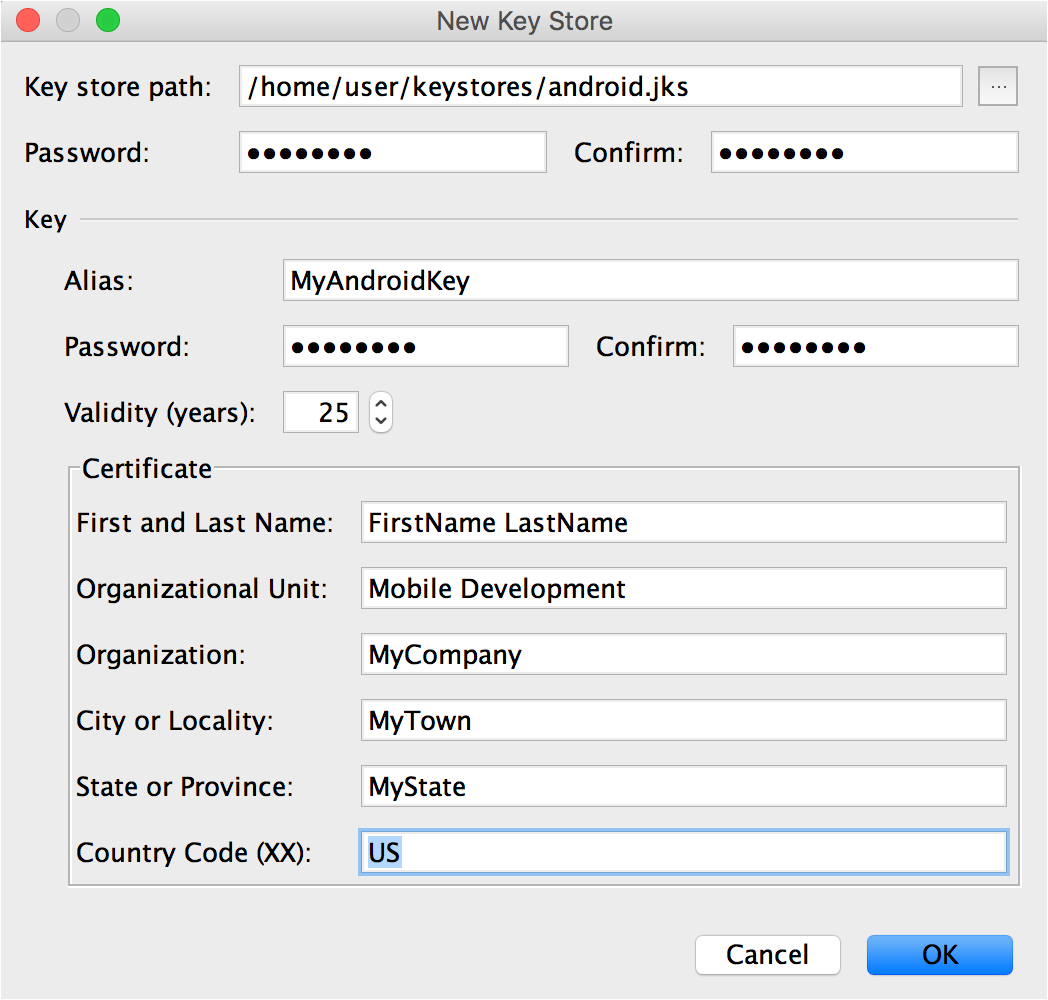
\includegraphics[width=0.7\textwidth]{inc/img/new_keystore.png}
  \caption{Создание нового ключа и хранилища ключей}
  \label{fig:newKeystore}
\end{figure}

В верхнем меню нужно выбрать \code{Build > Generate Signed APK}, после чего выбрать модуль в выпадающем меню и нажать \code{Next}.
Если нужно создать новый ключ и хранилище, нужно нажать \code{Create new}.
Откроется окно \code{New Key Store} (см.~рисунок~\ref{fig:newKeystore}), в котором нужно заполнить все поля и нажать \code{OK}.

После того как хранилище ключей и ключ созданы, нужно настроить подпись приложения в Gradle.
Для этого сначала надо добавить конфигурацию подписи, а после, ссылку на неё в релизную конфигурацию сборки как это сделано в листинге~\ref{lst:signingConfig}.

\begin{listing}[h]
  \kotlinfile{inc/src/signingConfig.gradle.kts}
  \caption{Конфигурация подписи APK в Gradle}
  \label{lst:signingConfig}
\end{listing}

Чтобы сохранить в тайне пароль от ключа и хранилища ключей при использовании VCS, можно вынести эти настройки в отдельный файл \code{.properties}, который не будет включён в систему контроля версий, и считывать их из него перед подписью.
Важно, чтобы файл хранилища ключей ни в коем случае не был включён в систему контроля версий.

\subsection{Публикация приложения}
\label{subsec:publish}

Публикация приложения "--- это основная цель разработки, т.к.\ это процесс, который делает приложение доступным для пользователей.
До, непосредственно, публикации приложение нужно подготовить.
Помимо электронной подписи, как минимум нужно удалить из приложения логирование  и отладочные атрибуты из манифеста, а так же добавить атрибуты \code{android:versionCode} и \code{android:versionName}.
Android Gradle Plugin делает это автоматически при переключении в режим релизной сборки.
Так же, необходимо тщательно протестировать приложение как минимум на одном смартфоне и одном планшете с целевой версией Android.
Если приложение зависит от внешних сервисов, то нужно убедиться, что сервисы доступны, безопасны и готовы к работе~\cite{android:publish}.

Приложение можно опубликовать несколькими способами.
Обычно для публикации используют рынки приложений, но можно, так же, опубликовать приложение на своём сайте или рассылать его непосредственно пользователям.

Публикация на рынках приложений позволяет добиться максимального охвата аудитории, но это не всегда бывает нужно, например, на стадии разработки удобнее рассылать промежуточные сборки заказчику.

Главным рынком приложений является Google Play.
Это надёжная платформа для публикации, которая позволяет продавать или распространять бесплатно Android-приложения по всему миру.
При публикации приложения на Google Play, разработчик получает набор инструментов, позволяющих анализировать продажи, тенденции на рыке, следить за ошибками во время работы приложения и т.д.
Для публикации приложения на Google Play необходим аккаунт разработчика, для регистрации которого нужно заплатить 25 USD\@.

\subsection{Непрерывная интеграция}
\label{subsec:ci}

\Abbrev{CI}{continuous integration "--- непрерывная интеграция}
Непрерывная интеграция (CI) "--- это практика разработки, когда интеграция между членами команды происходит часто и при небольших изменениях кода, а не только в конце цикла разработки.
Целью является создание более здорового программного обеспечения путем разработки и тестирования с небольшими приращениями.

В качестве платформы непрерывной интеграции выбран Travis CI, так как он поддерживает сборку Android-проектов, является открытым, бесплатным для Open Source проектов и не требует установки на собственный сервер.
Travis CI поддерживает процесс разработки, автоматически собирая и тестируя приложения, как только обнаруживает изменения кода в VCS репозитории и обеспечивает немедленную обратную связь об успехе или неудаче изменений~\cite{travis:docs}.

\Abbrev{YAML}{YAML Ain't Markup Language "--- YAML -- не язык разметки}
Travis CI хранит настройки в файле \code{.travis.yml} в формате YAML\@.
Для сборки Android-приложения нужно указать настройки, аналогично тому как они указаны в листинге~\ref{lst:travisAndroid}.

\begin{listing}[h]
  \yamlfile{inc/src/travisAndroid.yml}
  \caption{Файл конфигурации Travis CI для сборки Android-проекта}
  \label{lst:travisAndroid}
\end{listing}

Сборка может быть долгой из-за того, что Travis CI каждый раз собирает приложение ``с чистого листа''.
То есть каждый раз создаётся виртуальное окружение, в котором устанавливается JDK, подтягиваются зависимости и т.д., а значит кэширование Gradle не работает.
Чтобы ускорить сборку, можно включить кэширование, для этого нужно указать в настройке \code{cache.directories} директории, которые используются для кэша (см.~листинг~\ref{lst:travisCache}).

\begin{listing}[h]
  \yamlfile{inc/src/travisCache.yml}
  \caption{Настройки Travis CI для сохранения кэша Gradle и Android}
  \label{lst:travisCache}
\end{listing}

Удобно использовать сервисы CI для сборки и публикации промежуточных версий приложения при разработке.
Для того, чтобы настроить автоматическую публикацию приложения в GitHub Releases нужно немного изменить сценарий сборки, а именно, нужно организовать подпись приложения, при этом не скомпрометировав ключ подписи.
Для этого в Travis CI предусмотрены инструменты шифрования, которые позволяют безопасно добавлять чувствительные данные в VCS репозиторий, не боясь утечки.

Travis CI использует асимметричный алгоритм шифрования и создаёт пару RSA ключей для каждого репозитория.
Публичный ключ доступен всем, а приватный ключ Travis CI хранит в тайне, таким образом любой пользователь может зашифровать данные публичным ключом, но расшифровать их сможет только Travis CI\@.

\Abbrev{CLI}{command line interface "--- интерфейс командной строки}
Для упрощения шифрования данных есть утилита Travic CLI\@.
Чтобы зашифровать файл достаточно авторизоваться и написать одну команду:
\codeline{sh}{$ travis encrypt-file <имя_файла> --add}
После чего файл будет зашифрован и настройки для его расшифровки будут автоматически добавлены в файл конфигурации \code{.travis.yml}.

Может понадобиться зашифровать не только файл, но и строковое значение, которое нужно указать в конфиге, например токен доступа к API GitHub для публикации релиза.
Для такого случая вместо команды \code{encrypt-file} нужно использовать команду \code{encrypt}, например:
\codeline{sh}{$ travis encrypt "токен_доступа"}
Полученное значение можно использовать в настройках, оно будет автоматически расшифровано.

\begin{figure}[ht]
  \centering
  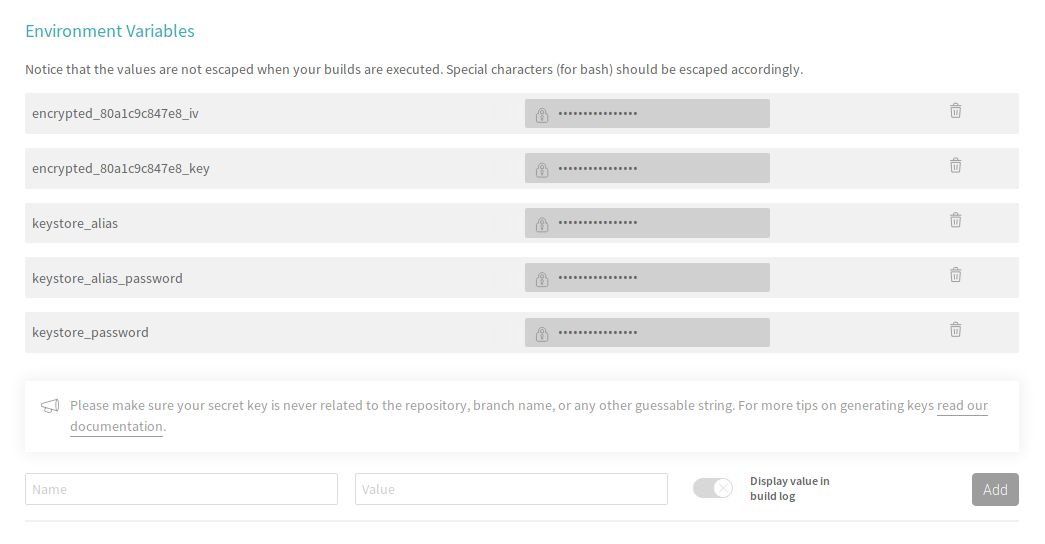
\includegraphics[width=\textwidth]{inc/img/travis_env.png}
  \caption{Веб-интерфейс Travis CI для добавления переменных окружения}
  \label{fig:travisEnv}
\end{figure}

Другой способ безопасного добавления строковых констант "--- добавление их через веб-интерфейс Travis CI (см.~рисунок~\ref{fig:travisEnv}), где нужно просто написать название переменной окружения, её значение и отключить отображение значения переменной в логах.
Этот способ проще, чем шифровка значений при помощи утилиты.

Для подписи приложения, нужно алиас ключа, пароль от ключа и пароль от хранилища ключей поместить в переменные окружения, а сам файл хранилища ключей зашифровать и добавить в систему контроля версий.
После того как эти действия выполнены, надо изменить конфигурацию подписи, чтобы при сборке из Travis CI конфигурации подписи брались из переменных окружения.
Результат можно увидеть в листинге~\ref{lst:ciSigning}.

\begin{listing}[h]
  \kotlinfile{inc/src/ciSigning.gradle.kts}
  \caption{Конфигурация подписи приложения}
  \label{lst:ciSigning}
\end{listing}

После того как приложение успешно подписывается, можно настроить автоматическую публикацию его в GitHub Releases.
Для этого в Travis CI есть секции \code{deploy} и \code{before\_deploy}.
Пример настроек с пояснениями приведен в листинге~\ref{lst:travisDeploy}

\begin{listing}[h]
  \yamlfile{inc/src/travisDeploy.yml}
  \caption{Настройки Travis CI автоматической публикации приложения}
  \label{lst:travisDeploy}
\end{listing}

\section{Тестирование и отладка в Android разработке}
\label{sec:testing}

\subsection{Методы тестирования программного обеспечения}
\label{subsec:testing:methods}

\subsection{Методология разработки TDD}
\label{subsec:testing:tdd}

\subsection{Тестирование пользовательского интерфейса}
\label{subsec:testing:ui}

\subsection{Отладка в IntelliJ IDEA}
\label{subsec:debug}

\conclusions
\label{sec:techConclusions}
